
\subsection{Layer Hardware}
ESP 32

\subsection{Layer Operating System}
Mongoose OS

\subsection{Layer Software Dependencies}
Django 3.0 Web framework
Bluetool


\subsection{Motor commands}
Receive Bluetooth commands and turn the corresponding shutters

\begin{figure}[h!]
	\centering
 	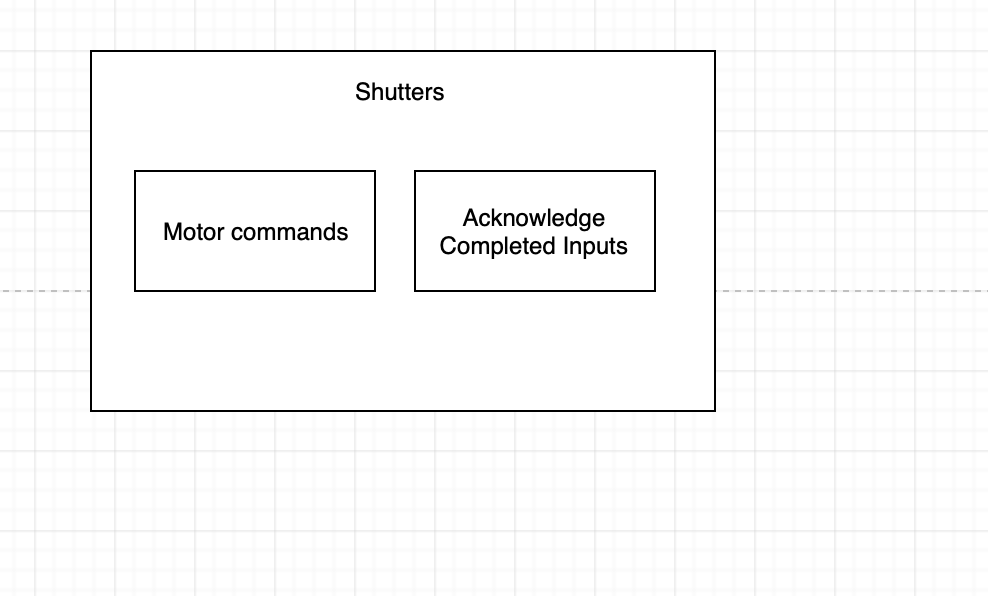
\includegraphics[width=0.60\textwidth]{images/Shutters}
 \caption{Example subsystem description diagram}
\end{figure}

\subsubsection{Subsystem Hardware}
ESP32

\subsubsection{Subsystem Operating System}
Mongoose OS

\subsubsection{Subsystem Software Dependencies}
Django 3.0 Web framework
Bluetool

\subsubsection{Subsystem Programming Languages}
C and micro python

\subsubsection{Subsystem Data Structures}
When the esp32 is given a request it will complete the request and send a message back to the original sender

\subsubsection{Subsystem Data Processing}
Esp32 will receive request and complete the request and send an acknowledgment 

\subsection{Acknowledge Completed Request}
Acknowledge completed Bluetooth commands

\subsubsection{Subsystem Hardware}
ESP32

\subsubsection{Subsystem Operating System}
Mongoose OS

\subsubsection{Subsystem Software Dependencies}
Bluetooth module working and request be formatted properly


\subsubsection{Subsystem Programming Languages}
C and micro python

\subsubsection{Subsystem Data Structures}
After the packets are received the shutter will try to complete the task and send a message back to original sender 

\subsubsection{Subsystem Data Processing}
Input checking making sure the input is properly formatted and checks to see if the new position does not equal the current position





